\documentclass{CLGPY}


\usepackage{listings}
\usepackage{cncolours}
\lstset{
    basicstyle=\small\ttfamily,%整体格式设置
    columns=fullflexible,%设置字符列为非等宽
    breaklines=true,%自动换行
    % frameround=ttff,%边框四角弧度,t则弧
    frame=tb,%边框样式
    backgroundcolor=\color{赤金!15},%背景颜色
    framerule=1.5pt,%边框线宽度
    rulecolor=\color{墨色},%边框线颜色
    % framesep=.5em,%边距
    numbers=left,%左边显示数字
    % numbersep=0em,
    xleftmargin=2em,
    framexleftmargin=2em,
    numberstyle={\sffamily\footnotesize\color{teal}}
}

\lstdefinelanguage{latex}{
    morecomment=[l]{\%},
    commentstyle=\color{lightgray},
    morekeywords={begin,end},
    keywordstyle=\color{blue!50!black},
    morekeywords={[2]documentclass,usepackage},%导言区命令
    keywordstyle={[2]\color{red!75!black}},
    morekeywords={[3]juanqi,title,author,institute,sxrq,jjxm,zzjj,txzz,xinxi,Title,Author,Institute,keywords,enkeywords,document,abstract,enabstract,minipage,tabular,tikzpicture,multicols,includegraphics,caption,captionof,center,quad,qquad,parbox,centering,subcaption,animateinline,bibliographystyle,cite,nocite,bibliography,textbf,enumerate,itemize,toprule,bottomrule,midrule,thebibliography,bibitem,small,footnotesize,verb},%命令和环境
    keywordstyle={[3]\color{cyan!70!black}},
    morekeywords={[4]maketitle,Maketitle,figure,table},
    keywordstyle={[4]\color{朱红}},
    morekeywords={[5]CLGPY,ctexart,ctexbook,ctexrep,book,article,report,standalone,tikz,tikz-3dplot,animate,ctex,fontspec,multicol,caption,subcaption,natbib,float,booktabs,geometry,graphicx,color,xcolor,hyperref,amsmath,mathtools,siunitx,mathabx},%文类和宏包
    keywordstyle={[5]\color{竹青}},
    morekeywords={[6]part,chapter,section,subsection,subsubsection,paragraph,subparagraph},%章节
    keywordstyle={[6]\color{琥珀}},
    morekeywords={[7],newcommand,newenvironment,renewcommand,renewenvironment,def,edef,gdef,xdef}%定义类命令
    keywordstyle={[7]\color{blue!70!black}},
}
\lstnewenvironment{latexcode}
{\lstset{language=latex}}
{}%代码设置,定义了用来排版LaTeX代码的latexcode环境
%%---------------------字体设置--------------------%

% 注意:如果希望使用\ctexset 在导言区指定字库,则需要先在宏包/文档类选项中指定fontset = none(这会禁用CTEX 宏集的操作系统检测功能和自动设定字库功能)
\setCJKmainfont[ItalicFont={FZKai-Z03},BoldFont={FZHei-B01},BoldItalicFont=FZLiShu-S01S]{FZShuSong-Z01}%设置正文字体为宋体,其粗体为黑体、斜体为楷体、粗斜为隶书,全文的一种设置
\setCJKsansfont{FZHei-B01}%设置无衬线字体为黑体
% \setCJKmonofont{}%设置打字机字体
%设置字体族
\setCJKfamilyfont{zhsong}{FZShuSong-Z01}
\setCJKfamilyfont{zhhei}{FZHei-B01}
\setCJKfamilyfont{zhkai}{FZKai-Z03}
\setCJKfamilyfont{zhfs}{FZFangSong-Z02}
%带*的\newcommand*不能有\par
\def\songti{\CJKfamily{zhsong}} % 宋体
\def\heiti{\CJKfamily{zhhei}} % 黑体
\def\kaishu{\CJKfamily{zhkai}} % 楷书
\def\fangsong{\CJKfamily{zhfs}} % 仿宋
%--------------------------------------------------%%字体设置
%--------------------以下命令是为了写说明文档而定义的,实际使用时可不管------------------------------%
\def\ts#1{\textcolor{red}{#1}}%提示命令
\def\bzx#1#2{$\underbracket[.5pt][1pt]{\text{#1}}_{\textcolor{red}{\text{#2}}}$}%下标注命令
\def\bzs#1#2{$\overbrace{\text{#1}}^{\textcolor{red}{\text{#2}}}$}%上标注命令
% \def\xbz#1#2{\vtop{\halign{##\crcr \hfil #1\hfil\crcr \noalign{\nointerlineskip\textcolor{red}{\hrule}\kern1pt} \hfil\small\textcolor{red}{#2}\hfil\crcr}}}%一个失败的尝试
\def\BibTeX{{%
\rm
B%
\kern-.05em%
{%
\sc
i%
\kern-.025em %
b%
}%
\kern-.08em
T%
\kern-.1667em%
\lower.7ex\hbox{E}%
\kern-.125em%
X%
}}%bibtex样式定制%为了写说明文档而定义的几个命令

%--------------------------使用说明----------------------%
%注:\juanqi、\title、\author三条命令必须要有,不然系统会终止编译
\juanqi{X}{X}%卷期填写,命令\juanqi{<卷>}{<期>}
\title[论文题目]{论文题目\ts{(20字以内,小二黑体)}}%标题填写,命令\title[<想要出现在奇数页页眉的标题,若缺省则默认为正式标题>]{<正式标题>}
\author[张某某,等]{张某某\textsuperscript{1},李\kern\ccwd 某\textsuperscript{2}\ts{(小四仿宋)}}%作者填写,命令\author[<想要出现在奇数页页眉的作者,若缺省则默认为正式作者>]{<正式作者>}
\institute{({1.云南大学{\kern.5\ccwd} 物理与天文学院,云南{\kern.5\ccwd}昆明 650504};2.……)\ts{(六号宋体)}}%机构填写,命令\institute{<机构>}

\begin{document}
    \maketitle%生成题名页并修改题名页页眉

    \sxrq{2021--1--1}{2021--1--3}%收稿、修改日期,命令\sxrq{<收稿日期>}{<修改日期>}
    \jjxm{XXXXXX基金(xxxxxxxx)资助}%基金项目,命令\jjxm{<基金项目>}
    \zzjj{XXX(2000 —),男,云南昆明人,云南大学物理系本科生,主要从事物理方面的工作.\ts{(第一作者)}}%第一作者简介,命令\zzjj{<第一作者简介>}
    \txzz{X X,E–mail: \url{XXXXX@ynu.edu.cn}}%通讯作者,命令\txzz{<通讯作者>}

    \begin{abstract}%中文摘要环境
        中文摘要文字须\emph{200字}左右,重点包括4个要素,即论文中心思想、方法、结果和结论.方法与结果部分应有必要的数据.摘要须用第三人称撰写,不引用参考文献、图表、数学公式和化学式.\ts{(``摘要''小五黑体,正文小五宋体)}
    \end{abstract}
    \keywords{模板说明;使用样例\ts{(``关键词''小五黑体;具体内容小五宋体,$3\sim 5$个)}}%中文关键词命令

    \xinxi{O 4–1\ts{(参照:\url{http://www.ztflh.com}})}{\bzx{A}{作者抄写}}{\bzx{1000-0712}{作者抄写} \bzx{XXXXXX}{编辑填写}}{\bzx{10.16854/j.cnki.1000-0712.}{作者抄写} \bzx{XXXXXX}{编辑填写}}%一些必要信息填写,命令\xinxi{<中图分类号>}{<文献标识码>}{<文章编号>}{<【DOI】>}

    \begin{multicols}{2}%以下部分内容采用双栏排版
        引言部分不需写标题,即不写“引言”二字.参考文献序号按其在文中出现的顺序编排,文中引用处用上标\cite{xingshinianfenlun,li2000yi},3个以上用连字符\cite{xingshinianfenlun,li2000yi,CTEX}.全文数字、西文用Times New Roman(\ts{已设定}),句号用实心点.

        \section{基本使用说明\ts{(一级标题小四黑体)}}
        \subsection{中文排版要求\ts{(二级标题五号黑体)}}
        源代码须保存为UTF-8 编码,并使用xelatex编译.

        \subsection{几个命令的新增与变动}
        本文类是在\verb|ctexart|文类的基础上改造的,相对于原文类,变动并新增了部分命令.题名页新增命令为:\verb|\juanqi|、\verb|\institute|,去除了\verb|\date|命令,日期自动生成在标题页页眉左(中文)右(英文).此外,对于题名页,\verb|\juanqi|、\verb|\title|、\verb|\author|三条命令必须要有,不然系统会终止编译并给出相应错误信息,其中\verb|\title|和\verb|\author|都各自提供了一个可选参数\verb|[<opttions>]|,用来填写想要出现在奇数页页眉的标题和作者,若缺省则默认为正式标题和正式作者(强烈建议自己填写\verb|[<options>]|,以免出现默认值过于冗长而造成页眉拥挤的情况).填写完基本信息后,使用\verb|\maketitle|命令即可生成标题页,顺便更改标题页所在页眉样式,代码如下:

        \begin{latexcode}
     \documentclass{CLGPY}
     %导言区
     \juanqi{<卷>}{<期>}
     \title[<options>]{<正式标题>}
     \author[<options>]{<正式作者>}
     \institute{<机构>}
     \begin{document}
     %正文区
         \maketitle
         ……
     \end{document}
        \end{latexcode}

        接下来可填写必要脚注信息,这些也是新增命令(为保证\emph{在标题页生成必要脚注信息},强烈建议将这几条代码写在文档靠前部分):
        \begin{latexcode}
         ……
         \sxrq{<收稿日期>}{<修改日期>}
         \jjxm{<基金项目>}
         \zzjj{<第一作者简介>}
         \txzz{<通讯作者>}
         ……
        \end{latexcode}

        按官方论文模板格式内容的先后顺序要求,下面要填的自然是摘要、关键词和一些必要信息.其中,摘要内容在\verb|abstract|环境中填写,关键词在\verb|\keywords| 命令中填写,必要信息在\verb|\xinxi|命令中填写,代码如下:%(注:命令中参数内容可空置但不可少大括号\{\})
        \begin{latexcode}
         ……
         \begin{abstract}
             摘要内容
         \end{abstract}
         \keywords{<具体关键词>}
         \xinxi{<中图分类号>}{<文献标识码>}%
               {<文章编号>}{<【DOI】>}
         ……
        \end{latexcode}

        \subsection{分栏与正文填写}
        上一部分所说内容填写完成后,接下来便可正式填写文章内容了,正文采用双栏排版,使用\verb|multicol|宏包提供的\verb|multicols|环境即可实现.此外,一级标题和二级标题分别使用\verb|\section|、\verb|\subsection|来填写,即:%本文类已调用multicols宏包,、三级标题使用\verb|\subsubsection|填写
        \begin{latexcode}
         ……
         \begin{multicols}{2}%分成两栏
             引言部分…… %空行分段

             \section{<一级标题>}
             一级标题内容
             \subsection{<二级标题>}
             二级标题内容
             ……
         \end{multicols}
         ……
        \end{latexcode}

        \subsection{英文部分的填写}
        与中文标题填写类似,使用\verb|\Title|、\verb|\Author|、\verb|\Institute|命令声明英文标题、作者、机构(注意命令首字母都是大写),再使用\verb|\Maketitle|命令生成标题信息,如下:
        \begin{latexcode}
         ……
         \Title{<英文标题>}
         \Author{<英文作者>}
         \Institute{<英文机构>}
         \Maketitle %生成标题信息
         ……
        \end{latexcode}

        填写完英文标题信息后,接下来便是在\verb|enabstract|环境中填写英文摘要,在\verb|\enkeywords| 命令中填写英文关键词,如下:
        \begin{latexcode}
         ……
         \begin{enabstract}
             英文摘要
         \end{enabstract}
         \enkeywords{<英文关键词>}
         ……
        \end{latexcode}

        \subsection{基本文档内容}
        总的来说,对于此文类,一份基本的文档内容应包括以下内容:
        \begin{latexcode}
     \documentclass{CLGPY} %使用CLGPY文类
     %导言区
    
     \juanqi{<卷>}{<期>}%卷期声明
     \title[<options>]{<正式标题>}%标题声明
     \author[<options>]{<正式作者>}%作者声明
     \institute{<机构>}%机构声明
     \begin{document}
     %正文区
         \maketitle %生成标题信息

         \sxrq{<收稿日期>}{<修改日期>}
         \jjxm{<基金项目>}
         \zzjj{<第一作者简介>}
         \txzz{<通讯作者>}

         \begin{abstract}
            摘要内容
         \end{abstract}
         \keywords{<具体关键词>}
         \xinxi{<中图分类号>}{<文献标识码>}%
               {<文章编号>}{<【DOI】>}
         
         \begin{multicols}{2} %分成两栏
             引言部分…… %空行分段
   
             \section{<一级标题>}
             一级标题内容
             \subsection{<二级标题>}
             二级标题内容
             ……
             参考文献
         \end{multicols}

         \Title{<英文标题>}
         \Author{<英文作者>}
         \Institute{<英文机构>}
         \Maketitle %生成标题信息

         \begin{enabstract}
            英文摘要
         \end{enabstract}
         \enkeywords{<英文关键词>}

     \end{document}
        \end{latexcode}

        \section{插图指南}
        插图需要用到\verb|graphicx|宏包(本文类已调用)的\verb|\includegraphics[<选项>]{<文件名>}|命令来实现,若图形文件与\verb|.tex|源文件在同一目录,则可直接填写文件名(可省略文件拓展名),若不在同一目录,需用路径指明图形文件所在位置(相对路径或绝对路径均可,路径用斜线\verb|/|分隔),例如相对于源文件,在路径\path{./fig/lion/lion.png}下有一张狮子图片,则插入命令应为:
        \begin{latexcode}
    ……
\includegraphics[scale=.5]%
    %将图片缩放到原来的0.5倍
    {./fig/lion/lion.png}%图片路径
    ……
        \end{latexcode}
        于是便可得到\autoref{fig:lion}所示的狮子图形.
        \begin{center}
            \includegraphics[scale=.5]{./fig/lion/lion.png}
            \captionof{figure}{\TeX{}狮子\label{fig:lion}}
        \end{center}
        
        此外,可选项可用\verb|width|、\verb|height|、\verb|scale|、\verb|angle|来设置图形的宽度、高度、缩放比例以及其逆时针旋转的角度,具体说明见\autoref{tab:ctxx}.
        \begin{center}
            \captionof{table}{\textbackslash includegraphics命令常用可选参数说明\label{tab:ctxx}}
            \begin{tabular}{>{\footnotesize}c>{\footnotesize}c}
                \toprule
                \textbf{参数}            &       \textbf{含义} \\
                \midrule
                \verb|width|$=<width>$   &  设置图片宽度为$<width>$ \\
                \verb|height|$=<height>$ &  设置图片高度为$<height>$\\
                \verb|scale|$=<scale>$   &  将图片缩放为原来的$<scale>$倍 \\
                \verb|angle|$=<angle>$   &  将图片逆时针旋转$<angle>$度 \\
                \verb|origin=l/r/c/t/b/B|&  指明旋转中心(左/右/中/上/下/基线)  \\
                \bottomrule
            \end{tabular}
        \end{center}
        
        \subsection{直接插图}
        不使用浮动体直接插图,可借助\verb|caption|宏包(本文类已调用)中的\verb|\captionof{<类型>}{<标题>}| 命令来生成题注.另外值得一提的是\verb|\linewidth|命令,它表示当前文本行的宽度,\emph{在不同环境中会有所不同}(在后面的例子中会看到它的作用),可借助它配合插图命令使用,例如下面代码:
        \begin{latexcode}
\begin{center}% center环境让图形居中排版
   \includegraphics[width=.7\linewidth]%
              {example-image}%图形文件名
   \captionof{figure}{插图示例——直接插图}
\end{center}
        \end{latexcode}
        便可得到\autoref{fig:zjct}(图形宽度为行宽的$0.7$倍):
        \begin{center}
            \includegraphics[width=.7\linewidth]{example-image}
            \captionof{figure}{插图示例——直接插图\label{fig:zjct}}
        \end{center}

        \subsection{使用浮动体}
        \LaTeX{}预定义了\verb|figure|和\verb|table|两类浮动体环境,通常为\verb|figure|里放图片,\verb|table|里放表格,以\verb|figure|为例,代码如下:
        \begin{latexcode}
         \begin{figure}[<允许位置>]
            ……
         \end{figure}
        \end{latexcode}
        \verb|<允许位置>|参数用来设定浮动体允许排版的位置,通常有\verb|h、t、b、p、!|及其组合.经测试,这几个常用的参数在\verb|multicols|环境中会使图表莫名消失,目前的解决方法是使用\verb|float|宏包提供的\verb|<H>|位置选项在浮动体中产生没有浮动效果的图表环境(也就是图表会显现在\emph{当前位置}而不会“乱跑”),这样图表便可正常显现出来.例如,下面代码:
        \begin{latexcode}
 \begin{figure}[H]
   \centering %使图片居中排版
   \includegraphics[scale=.5,angle=90]%
                   {example-image-a}
   \caption{插图示例——浮动体环境插图}
 \end{figure}
        \end{latexcode}
        可得到\autoref{fig:fdt}(将图片缩放到原来的$0.5$倍,并旋转$90\du$):
        \begin{figure}[H]
            \centering
            \includegraphics[scale=.5,angle=90]{example-image-a}
            \caption{插图示例——浮动体环境插图\label{fig:fdt}}
        \end{figure}

        \subsection{并排和子图表}
        在一个浮动体里面放置多张图片,大致可分为三种情况:
        \begin{enumerate}
            \item 多图共用一个标题;
            \item 多图拥有各自的标题;
            \item 多图有各自的子标题,同时共用一个大标题.
        \end{enumerate}
        下面分别举例:

        对于第一种情况,也是最简单的情况,直接并排放置即可,可以通过分段或者换行命令\verb|\\| 排版多行图片,例如下面代码:
        \begin{latexcode}
\begin{figure}[H]
   \centering
   \includegraphics[width=.47\linewidth]%
                {example-image-a}
   \includegraphics[width=.47\linewidth]%
                {example-image-b}\\[3pt]%
                %换行并增加3pt的垂直间距
   \includegraphics[width=.47\linewidth]%
                {example-image-b}
   \includegraphics[width=.47\linewidth]%
                {example-image-a}
   \caption{多图共用一个标题}
\end{figure}
        \end{latexcode}
        便可得到\autoref{fig:dtgy}(每张图形宽度为行宽的$0.47$倍):
        \begin{figure}[H]
            \centering
            \includegraphics[width=.47\linewidth]{example-image-a}
            \includegraphics[width=.47\linewidth]{example-image-b}\\[3pt]
            \includegraphics[width=.47\linewidth]{example-image-b}
            \includegraphics[width=.47\linewidth]{example-image-a}
            \caption{多图共用一个标题\label{fig:dtgy}}
        \end{figure}

        对于第二种情况,可以借助\verb|\parbox|或\verb|minipage| 生成段盒子,将标题限制在盒子内来实现,\verb|\parbox| 和 \verb|minipage| 环境的语法格式如下:
        \begin{latexcode}
\parbox[<盒子基线位置>]%默认值为c
%位置参数可用c(居中)、t(顶部)、b(底部)表示
       [<盒子高度>]%
       [<指定高度后盒子内容在盒子内的位置>]%
%内容位置参数可用c/t/b/s(垂直分散对齐)表示
       {<盒子宽度>}{<盒子内容>}
%可选参数[<options>]缺省会有其默认值
        \end{latexcode}
        \begin{latexcode}
\begin{minipage}[<盒子基线位置>]%默认c
                [<盒子高度>][<内容位置>]%
                {<盒子宽度>}
    <盒子内容>
\end{minipage}
        \end{latexcode}
        对于前面所说情况,例如下面代码:
        \begin{latexcode}
\begin{figure}[H]
   \centering
   \begin{minipage}{.47\linewidth}
     \centering
     \includegraphics[width=\linewidth]%
                     {example-image-a}
     \caption{并排图1}
   \end{minipage}
   \quad%间隔1em
   \begin{minipage}{.47\linewidth}
     \centering
     \includegraphics[width=\linewidth]%
                     {example-image-b}
     \caption{并排图2}
   \end{minipage}
\end{figure}
        \end{latexcode}
        可得到\autoref{fig:bp1}和\autoref{fig:bp2}:
        \begin{figure}[H]
            \centering
            \begin{minipage}{.47\linewidth}
                \centering
                \includegraphics[width=\linewidth]{example-image-a}
                \caption{并排图1\label{fig:bp1}}
            \end{minipage}
            \quad
            \begin{minipage}{.47\linewidth}
                \centering
                \includegraphics[width=\linewidth]{example-image-b}
                \caption{并排图2\label{fig:bp2}}
            \end{minipage}
        \end{figure}

        对于第三种情况,同样可借助段盒子(或小页环境)来实现,再利用\verb|subcaption|宏包提供的\verb|\subcaption| 命令生成子标题,同时用\verb|\caption|加上整体的标题,例如:
        \begin{latexcode}
\begin{figure}[H]
   \centering
   \parbox[b]{.47\linewidth}{\centering%
       \includegraphics[width=\linewidth]%
                       {example-image-a}
       \subcaption{子图1}}%注意括号要配对
   \parbox[b]{.47\linewidth}{\centering%
   \includegraphics[width=\linewidth]%
                   {example-image-b}
   \subcaption{子图2}}%注意括号要配对
   \caption{插图示例——并排插图}
\end{figure}
        \end{latexcode}
        可得到子图\ref{fig:zt1}和子图\ref{fig:zt2},它们拥有共同的标题:\nameref{fig:gbt}:%\nemeref命令可用来引用文章的章节标题和图表标题
        \begin{figure}[H]
            \centering 
            \parbox{.47\linewidth}{\centering\includegraphics[width=\linewidth]{example-image-a}\subcaption{子图1\label{fig:zt1}}} 
            \parbox{.47\linewidth}{\centering\includegraphics[width=\linewidth]{example-image-b}\subcaption{子图2\label{fig:zt2}}}
            \caption{插图示例——并排插图\label{fig:gbt}}
        \end{figure}
         此外,\verb|subcaption|宏包还提供了\verb|subfigure|和 \verb|subtable|环境,其语法功能与\verb|minipage|完全相同,不同之处在于可直接在其里面使用\verb|\caption|命令来生成子标题,此处不表.
        
         关于插图,最后要说的是,插图方式不固定,怎么好用怎么用,例如还可使用\verb|easyfloats|等宏包来排版浮动体,请自行查阅相关手册.
       
        \section{绘图示例}
        \LaTeX{}除了用来排版文字,也可支持用代码绘制图形,此处给出两例:
        
        首先可利用\verb|tikz|宏包绘制函数$e^x$在$x=0$处的前三阶泰勒展开式示意图,具体代码参见源文件,此处不再展示,如\autoref{fig:zk2}所示:

%========================绘图示例代码===========================%
        \begin{figure}[H]
            \centering
            \begin{minipage}[b]{\linewidth}
                \centering
                \tikzset{gscale/.style={scale=#1,every node/.append style={scale=#1}}}%同步放大图形和节点
                 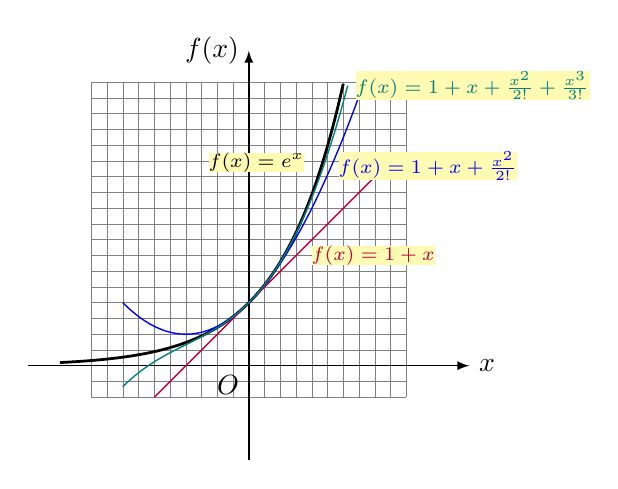
\begin{tikzpicture}[scale=.8,samples=100,line width=.5pt,m/.style={fill=yellow!30,outer sep=0pt,inner sep=0pt,font=\scriptsize}]
                     \draw[help lines,step=.25](-2.5,-.5)grid(2.5,4.5);
                     \draw[-latex](-3.5,0)--(3.5,0)node[right]{$x$};
                     \draw[-latex](0,-1.5)--(0,5)node[left]{$f(x)$};
                     \draw(0,0)node[below left]{$O$};
                     \draw [line width=1pt]  plot[domain=-3:1.5]      (\x,{e^(\x)})                             node[m,left,shift={(-.5,-1)}]{$f(x)=e^x$};
                     \draw [purple]          plot[domain=-1.5:2]      (\x,{1+\x})                               node[m,right,shift={(-.8,-1)}]{$f(x)=1+x$};
                     \draw [blue]            plot[domain=-2:1.8]      (\x,{1+\x+((\x)^2)/2!})                   node[m,right,shift={(-.3,-1)}]{$f(x)=1+x+\frac{x^2}{2!}$};
                     \draw [teal]            plot[domain=-2:1.57]     (\x,{1+\x+((\x)^2)/2!+(\x)^3/3!})         node[m,right,shift={(0.1,0)}]{$f(x)=1+x+\frac{x^2}{2!}+\frac{x^3}{3!}$};
                 \end{tikzpicture}
                 \caption{函数$e^x$在$x=0$处的前三阶泰勒展开式}
                 \label{fig:zk2}
             \end{minipage}
        \end{figure}
%==============================================================%

        此外,可用\verb|tikz|、\verb|tikz-3dplot|以及\verb|animate| 宏包绘制一个动点绕定点转动示意图(一般来说论文中不适宜有动图,此处只是卖弄一下\LaTeX{}的绘图功能),如\autoref{fig:drd}所示,具体代码参见源文件,此处仅给出大致代码:
        \begin{latexcode}
\documentclass{standalone}
%单独绘图建议选用standalone文类
%导言区调用相应宏包
\usepackage{ctex}%中文支持宏包
\usepackage{animate}%动图绘制宏包
\usepackage{tikz,tikz-3dplot}
\begin{document}
    %正文区开始绘图
    \begin{animateinline}%动图绘制环境
        \begin{tikzpicture}%具体图形绘制环境
            具体图形代码
        \end{tikzpicture}
    \end{animateinline}
\end{document}  
        \end{latexcode}
%========================绘图示例代码==========================%
% \usepackage{tikz,tikz-3dplot,animate}
%===========================================绘图示例代码==================================================%
%把绘图命令单独定义出来,使得后续方便使用animateinline环境
\newcommand{\drd}[3]{%
\tdplotsetmaincoords{67}{110}%调整坐标系角度
\begin{tikzpicture}[scale=3,tdplot_main_coords,t/.style={font=\scriptsize\itshape}]
    \def\R{.5}%圆周半径,单独定义出来易于修改
    \coordinate(O) at (0,0,0);%定原点,产生参考点
  
    %设置转动坐标系(Euler rotations)
    \tdplotsetrotatedcoords{#1}{#2}{#3}%#1为进动角,#2为章动角,#3为自转角;若没有\tdplotsetrotatedcoordsorigin{point}设置转动坐标系的原点的话则原点默认与主坐标系重合
    \tdplotdrawarc[fill=gray!15,line width=1pt,draw=blue!50!cyan,tdplot_rotated_coords]{(O)}{\R}{0}{360}{}{};%使用tdplot_rotated_coords切换到转动坐标系,并在转动坐标系中画一个圆轨道,圆弧命令:\tdplotdrawarc[coordinate system, draw styles]{(中心点)}{圆弧半径}{起始角}{终止角}{label options}{label}
    % \draw[teal,->,tdplot_rotated_coords] (O)--(.6,0,0)node[above]{$x'$};
    % \draw[teal,->,tdplot_rotated_coords] (O)--(0,.6,0)node[above]{$y'$};
	% \draw[teal,->,tdplot_rotated_coords] (O)--(0,0,.6)node[above]{$z'$};
    
    %画主坐标系,因涉及到颜色覆盖问题而在转动坐标系之后画
    \shade[ball color=teal!30] (O) node[left,t]{定点} circle (.5pt);
    \draw[-latex] (O)--(1.8,0,0) node[right]{$x$(cm)};
    \draw[-latex] (O)--(0,2,0) node[above]{$y$(cm)};
    \draw[-latex] (O)--(0,0,1.5) node[above]{$z$(cm)};
    \tdplotdrawarc[help lines,dashed,thick]{(O)}{\R}{0}{360}{}{};
	
    %将旋转坐标系中的点对应到主坐标系中(点在主坐标系中的各位置分量分别存放到:\tdplotresx,\tdplotresy,\tdplotresz中)
	\tdplottransformrotmain{0.5}{0}{0}%选择动点,此处选动点为旋转坐标系的x轴与轨道的交点(因为容易选,你也可以随意选。)另外注意:\tdplottransformmainrot{x}{y}{z}能将主坐标系中某一点对应到旋转坐标系中,且各分量放在与之同名的\tdplotresx,\tdplotresy,\tdplotresz中
    \shade[tdplot_rotated_coords,ball color=brown] (0.5,0,0) node[above,t]{动点} circle (.5pt);
    \fill (\tdplotresx,\tdplotresy,0) circle (.2pt);
	\draw[-latex,red] (0,0,0) -- (\tdplotresx,\tdplotresy,\tdplotresz)node[below right,t]{$\vec{r}=(\tdplotresx,\tdplotresy,\tdplotresz)$};
	\draw[dashed,red] (0,0,0) -- (\tdplotresx,\tdplotresy,0);
	\draw[dashed,red] (\tdplotresx,\tdplotresy,\tdplotresz) -- (\tdplotresx,\tdplotresy,0);

	%计算指定点与z轴的夹角theta以及与x轴的夹角phi,结果存储在宏\tdplotrestheta和\tdplotresphi中
	\tdplotgetpolarcoords{\tdplotresx}{\tdplotresy}{\tdplotresz}

    % 标记角
    \tdplotdrawarc[->,olive,t]{(O)}{0.1}{0}{\tdplotresphi}{anchor=north}{$\phi=\tdplotresphi^\circ$}
    \tdplotsetthetaplanecoords{\tdplotresphi}%将phi平面转换到theta平面上,旋转角为:phi
    \tdplotdrawarc[tdplot_rotated_coords,->,olive,t]{(O)}{0.2}{0}{\tdplotrestheta}{above}{$\theta=\tdplotrestheta^\circ$}%注意要用tdplot_rotated_coords切换到所谓的theta平面
\end{tikzpicture}}

%-------------进动、章动、自转----------------%
\begin{center}
\begin{animateinline}[loop,autopause,controls,]{5}
    \multiframe{72}{ijdj=0+5,izdj=0+5,izxj=0+5}{%
    % \edef\ijdj{\ijdj}
    % \edef\izdj{\izdj}
    % \edef\izxj{\izxj}
    \drd{\ijdj}{\izdj}{\izxj}}%如果无法正常使用此命令,可考虑将参数先用\edef展开
\end{animateinline}
\captionof{figure}{动点绕定点转动示意图(进动、章动、自转共存)\label{fig:drd}}
\end{center}

%-------------进动----------------%
        % \begin{animateinline}[loop,autopause,controls,]{10}
        %     \multiframe{120}{ijdj=0+3,izdj=10+0,izxj=0+0}{%为了区别自转,先章动10°
        %     % \edef\ijdj{\ijdj}
        %     % \edef\izdj{\izdj}
        %     % \edef\izxj{\izxj}
        %     \drd{\ijdj}{\izdj}{\izxj}}%如果无法正常使用此命令,可考虑将参数先用\edef展开
        % \end{animateinline}

%-------------章动----------------%      
        % \begin{animateinline}[loop,autopause,controls,]{10}
        %     \multiframe{120}{ijdj=0+0,izdj=0+3,izxj=0+0}{%
        %     % \edef\ijdj{\ijdj}
        %     % \edef\izdj{\izdj}
        %     % \edef\izxj{\izxj}
        %     \drd{\ijdj}{\izdj}{\izxj}}%如果无法正常使用此命令,可考虑将参数先用\edef展开
        % \end{animateinline}  

%-------------自转----------------%
        % \begin{animateinline}[loop,autopause,controls,]{10}
        %     \multiframe{120}{ijdj=0+0,izdj=10+0,izxj=0+3}{%为了区别进动,先章动10°
        %     \edef\ijdj{\ijdj}
        %     \edef\izdj{\izdj}
        %     \edef\izxj{\izxj}
        %     \drd{\ijdj}{\izdj}{\izxj}}%如果无法正常使用此命令,可考虑将参数先用\edef展开
        % \end{animateinline}     
%========================================================================================================%
%==============================================================%
        \section{三线表的绘制}
        三线表的绘制可借助\verb|booktabs|宏包(本文类已调用),此宏包提供了以下几个表线命令:
        \begin{itemize}
            \item \verb|\toprule|:画表格顶部粗线,其粗细可用\verb|\heavyrulewidth|设置;
            \item \verb|\midrule|:画表格中间分隔线,其粗细可用\verb|\lightrulewidth|设置;
            \item \verb|\bottomrule|:画表格底部粗线,其粗细可用\verb|\heavyrulewidth|设置;
            \item \verb|\cmidrule{<起>-<止>}|:画指定列的分隔线,其粗细可用\verb|\cmidrulewidth|设置.
        \end{itemize}
        有了这些命令,就可以在制表环境中用它们来取代\verb|\hline|和\verb|\cline|命令,并在合适的位置使用合适的画线命令画出“三线”,例如下面代码:
        \begin{latexcode}
\begin{center}%使表格居中,不使用浮动体环境
   \captionof{table}{\LaTeX{}表格列格式说明}%表名置于表格上方
   \begin{tabular}{>{\small}l>{\footnotesize}l}%列格式说明:两列,左对齐,同时使用array宏包提供的>{<内容>}(表示把<内容>插入其后所在列的开头)设置各列字体尺寸
     \toprule %画表格顶部粗线
     \textbf{列格式} & \textbf{\small 说明} \\%第一列标题加粗,第二列标题在加粗的同时把字体尺寸设为small,然后用\\换行
     \midrule %画表格中间分隔线
     \verb|l|   &   本列左对齐   \\
     \verb|c|   &   本列居中   \\
     \verb|r|   &   本列右对齐   \\
     \verb|p{<宽度>}|   &   指定列宽   \\
     \verb|||   &   绘制竖线   \\
     \verb|@{<内容>}|   &   自定义内容   \\
     \verb|*{<计数>}{<列格式说明>}|     &     给出\verb|<列格式说明>|的重复次数   \\
     \bottomrule %画表格底部粗线
   \end{tabular}
\end{center}
        \end{latexcode}
        可得到\autoref{tab:lgs}:
        \begin{center}%使表格居中,不使用浮动体环境
            \captionof{table}{\LaTeX{}表格列格式说明\label{tab:lgs}}%表名置于表格上方
            \begin{tabular}{>{\small}l>{\footnotesize}l}%列格式说明:两列并居中
                \toprule %画表格顶部粗线
                 \textbf{列格式}   &     \textbf{\small 说明}   \\%换行
                 \midrule %画表格中间分隔线
                \verb|l|   &   本列左对齐   \\
                \verb|c|   &   本列居中   \\
                \verb|r|   &   本列右对齐   \\
                \verb|p{<宽度>}|   &   指定列宽   \\
                \verb|||   &   绘制竖线   \\
                \verb|@{<内容>}|   &   自定义内容   \\%使用@{<内容>}时会消除表列间距再插入<内容>,可用@{}来消除单元格前后的间距
                \verb|*{<计数>}{<列格式说明>}|   &   给出\verb|<列格式说明>|的重复次数   \\
                \bottomrule %画表格底部粗线
            \end{tabular}
        \end{center}
        
        注意:官方论文模板格式要求\emph{表名置于表格上方},因此在制表时要注意表名的摆放位置.此外,本文类已按官方期刊论文模板要求对图表标题的字体和字号进行了设定,在使用时无需再对其进行更改.
                             
                     
                             
                           
        

        \section{参考文献处理}
        \subsection{自行书写参考文献列表}
        这是一种比较本的方法,要自己硬排参考文献(包括格式),具体方法是使用\verb|thebibliography|环境,每条参考文献由\verb|\bibitem|引导,代码如下:
        \begin{latexcode}
\begin{thebibliography}{<widest label>}%
    %<widest label> 用以限制参考文献序号宽度,通常设定为与参考文献条目一致
    \bibitem[<自定义参考文献序号>]%
            {<文献标签>} ……
    ……
\end{thebibliography}
        \end{latexcode}

        \subsection{\BibTeX(强烈建议用此方法)}
        \begin{enumerate}
            \item 首先填写一份数据库文件名为\verb|xxx.bib|的\BibTeX 数据库.
            \item 在\verb|.tex|源文件(例如本文档为\verb|main.tex|)中添加一些必要命令:
            \begin{enumerate}
		    	\item
		    使用命令\verb|\bibliographystyle{<bst>}| 指定样式文件,以此设定参考文献的格式,\verb|<bst>|为\verb|.bst|样式文件的名称,注意\emph{不要带.bst 扩展名}.
		    	\item
		    	在正文中引用参考文献:
		    	\begin{itemize}
                \item \verb|\cite{<要引用的文献>}|引用文献并列出被引用的文献;
		    	 \item \verb|\nocite{<未被引用的文献>}| 列出未被引用的文献;
		    	 \item \verb|\nocite{*}|让所有未被引用的文献都列出.
            \end{itemize}
              \item
              在需要列出参考文献的位置,使用\verb|\bibliography{<bib-name>}| 命令,其中\verb|<bib-name>| 是\BibTeX 数据库的文件名,注意\emph{不要带.bib 扩展名}.
             \end{enumerate}
             \item 编译,过程如下(以本文档为例,可略去扩展名):
             \begin{latexcode}
    xelatex   main.tex
    bibtex   main.aux
    xelatex   main.tex
    xelatex   main.tex
             \end{latexcode}
        \end{enumerate}
        
		 参考文献应是公开出版刊物,以便评审者、编者、读者查证.\ts{作者仅保留三位}.
%-----------------------显示参考文献------------------------%
        \bibliographystyle{thuthesis-numeric}%这里使用了清华大学学位论文模板样式,其与《大学物理》期刊官方论文模板要求一致
       		\nocite{*}%让所有未被引用的文献都列出
        \bibliography{./bib/clgpy}

    \end{multicols}%结束分栏

%-----------------------英文信息部分------------------------%
\Title{Essay topic \ts{(英文题目第1个字母大写,其余小写;小三加黑)}}
\Author{ZHANG Mou-mou, LI Mou \ts{(小四)} \\ \ts{\small (姓在前并全部大写,名的第1个字母大写,其余小写. 双名中间用连字符连接,多名作者用“,”隔开.)}}
\Institute{(College of Physics and Astronomy, Yunnan University, Kunming 650504, China)\ts{(内容和顺序与中文作者单位对应;小五)}}
\Maketitle
\begin{enabstract}
    The English abstract requires simple sentence structure, smooth sentences, complete meaning, and corresponding to the Chinese abstract. The abstract must be written in the third person, without citing references, diagrams, mathematical formulas and chemical formulas.
    英文摘要要求句型简单、语句顺畅、意义完整,且与中文摘要对应.摘要须用第三人称撰写,不引用参考文献、图表、数学公式和化学式.\ts{(``Abstract''五号加黑,正文五号)}
    
\end{enabstract}
\enkeywords{corresponding to Chinese keywords 与中文关键词对应\ts{(``Key words''五号加黑,具体Key words五号,首字母小写)}}


\end{document}